\documentclass[ignorenonframetext,11pt]{beamer}
%\documentclass[onesided]{article}
%\usepackage{graphicx}
%\usepackage{beamerarticle}

\usepackage{beamerthemesplit}
\usepackage{patchcmd}
\usepackage{tabulary}		% Support longer table cells
\usepackage{booktabs}		% Support better tables

\usepackage{subfigure}

\let\oldSubtitle\subtitle

\def\myauthor{Author}			% In case these were not included in metadata
\def\mytitle{Title}
\def\mykeywords{}
\def\mybibliostyle{plain}
\def\bibliocommand{}
\def\affiliation{University of Melbourne}
\def\myauthor{Claudine Chionh}
\date{2 March 2010}
\def\mydate{2 March 2010}
\def\event{LUV meeting}
\def\format{complete}
\def\latexxslt{beamer}
\def\theme{CambridgeUS}
\def\mytitle{Humanities computing}

\ifx\subtitle\undefined
\else
	\oldSubtitle{\subtitle}
\fi

\ifx\affiliation\undefined
\else
	\institute{\affiliation}
\fi

\ifx\event\undefined
\else
	\date[\mydate]{\mydate~ / \event }
\fi

\ifx\graphic\undefined
\else
	\pgfdeclareimage[height=0.75cm]{university-logo}{\graphic}
	\logo{\pgfuseimage{university-logo}}
\fi

\ifx\theme\undefined
\else
	\usetheme{\theme}
\fi


\AtBeginSubsection[]
{
   \begin{frame}
       \frametitle{Outline}
       \tableofcontents[currentsection,currentsubsection]
   \end{frame}
}

%\title{\mytitle}

% Show "current/total" slide counter in footer
\title[\mytitle\hspace{2em}\insertframenumber/
\inserttotalframenumber]{\mytitle}


\author{\myauthor}
\addtolength{\parskip}{\baselineskip}

\begin{document}
\frame{\setlength\parskip{0pt}\titlepage}


\section{Founders and Survivors}
\label{foundersandsurvivors}

\begin{frame}
\frametitle{The {\itshape Claudine}}
\label{theclaudine}

Woolwich 24/aug/1821 to Hobart 15/dec/1821 -- 113 days at sea


160 male convicts boarded, 159 survived/landed (not a bad record)



\end{frame}
		

\begin{frame}
\frametitle{Journal}
\label{journal}

\begin{figure}
	\label{journal}
	\begin{center}
	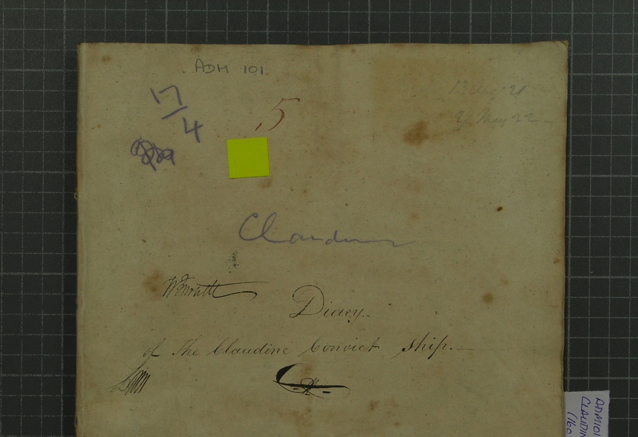
\includegraphics[keepaspectratio,width=\textwidth, height=.75\textheight]{images/claudine33.png}
	\end{center}
	\end{figure}
	



\end{frame}
		

\begin{frame}
\frametitle{Conduct registers}
\label{conductregisters}

\begin{figure}
	\label{johnastill}
	\begin{center}
	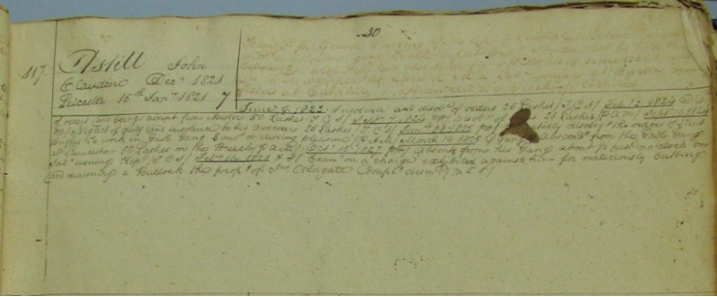
\includegraphics[keepaspectratio,width=\textwidth, height=.75\textheight]{images/Astill-cr.jpg}
	\end{center}
	\end{figure}
	



\end{frame}
		

\begin{frame}
\frametitle{Archives of Tasmania convict index}
\label{archivesoftasmaniaconvictindex}

\begin{figure}
	\label{convictsearch}
	\begin{center}
	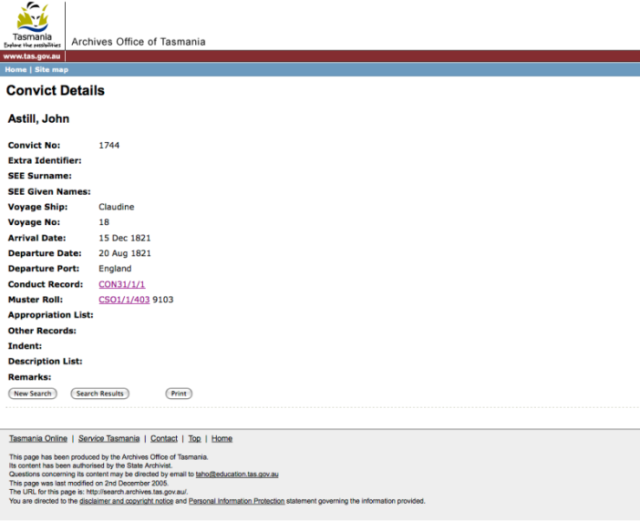
\includegraphics[keepaspectratio,width=\textwidth, height=.75\textheight]{images/Astill-aot.png}
	\end{center}
	\end{figure}
	



\end{frame}
		

\begin{frame}
\frametitle{Founders and Survivors}
\label{foundersandsurvivors}

\begin{figure}
	\label{foundersandsurvivors}
	\begin{center}
	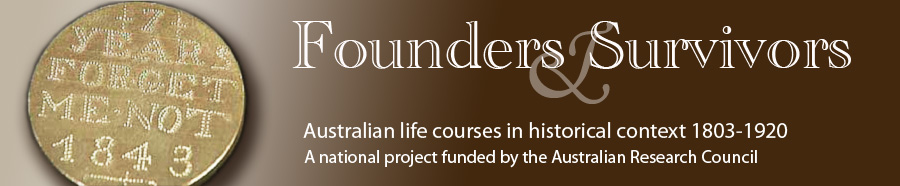
\includegraphics[keepaspectratio,width=\textwidth, height=.75\textheight]{images/logo.jpg}
	\end{center}
	\end{figure}
	



\end{frame}
		

\begin{frame}
\frametitle{Van Diemen's Land}
\label{vandiemensland}

Transportation period, 1803-1853


\ensuremath{\sim} 1 million rows of data


Quantifiable data: conduct registers, BDM{\ldots}


Text: journals, newspaper reports



\end{frame}
		

\begin{frame}
\frametitle{Genealogists}
\label{genealogists}

What happened to convicts after they were freed?


Links with genealogists for lives of convicts and their families.



\end{frame}
		

\begin{frame}
\frametitle{The `factory plan'}
\label{thefactoryplan}

\begin{figure}
	\label{factory}
	\begin{center}
	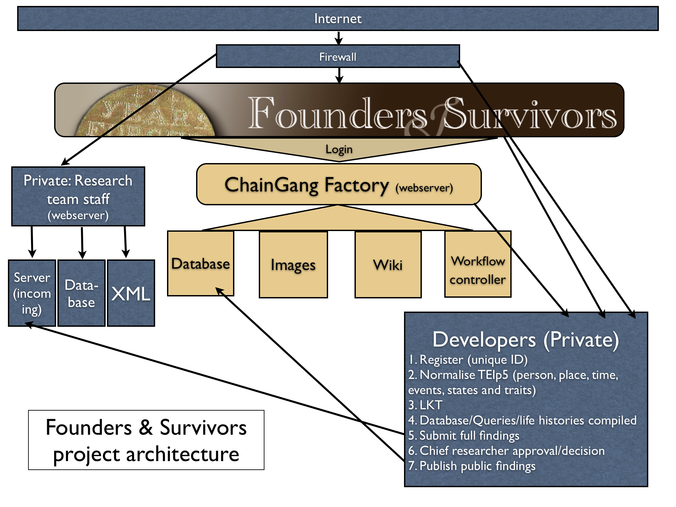
\includegraphics[keepaspectratio,width=\textwidth, height=.75\textheight]{images/factory33.png}
	\end{center}
	\end{figure}
	



\end{frame}
		

\section{Humanities computing}
\label{humanitiescomputing}

\begin{frame}
\frametitle{`Humanities computing'}
\label{humanitiescomputing}

Or `digital humanities'?



\end{frame}
		

\begin{frame}
\frametitle{Old questions, new tools?}
\label{oldquestionsnewtools}

Digitisation


Analyse large[r] amounts of material


Public access and collaboration



\end{frame}
		

\begin{frame}
\frametitle{The Valley of the Shadow}
\label{thevalleyoftheshadow}

\begin{figure}
	\label{letter}
	\begin{center}
	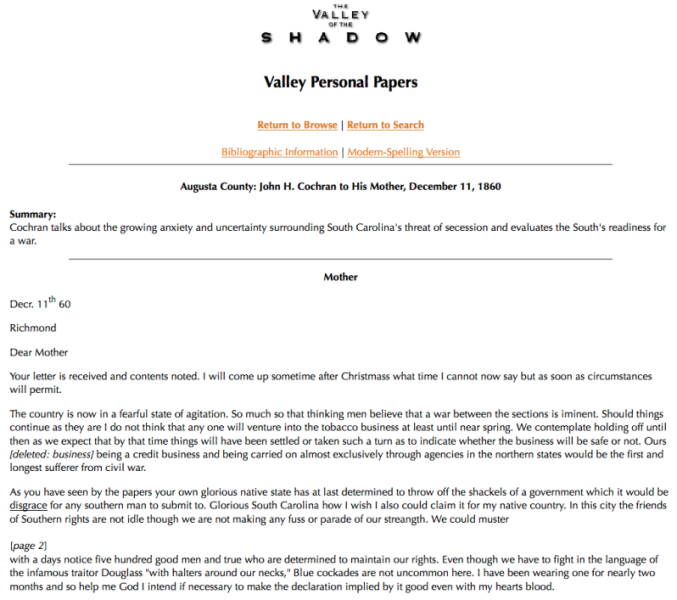
\includegraphics[keepaspectratio,width=\textwidth, height=.75\textheight]{images/valley.png}
	\end{center}
	\end{figure}
	



\end{frame}
		

\begin{frame}
\frametitle{The Valley of the Shadow}
\label{thevalleyoftheshadow}

\begin{figure}
	\label{map}
	\begin{center}
	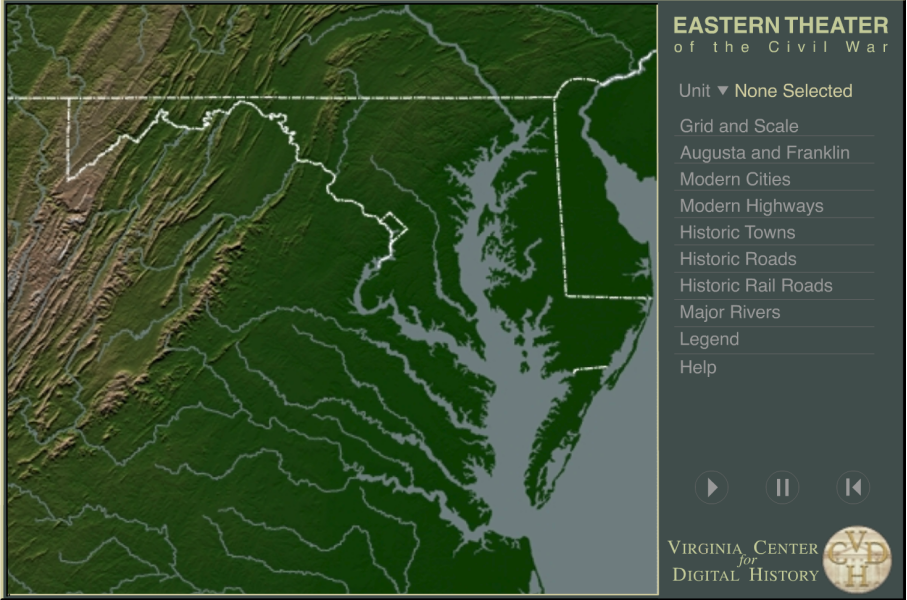
\includegraphics[keepaspectratio,width=\textwidth, height=.75\textheight]{images/battlemap.png}
	\end{center}
	\end{figure}
	



\end{frame}
		

\begin{frame}
\frametitle{Old Bailey Online}
\label{oldbaileyonline}

\begin{figure}
	\label{oldbailey}
	\begin{center}
	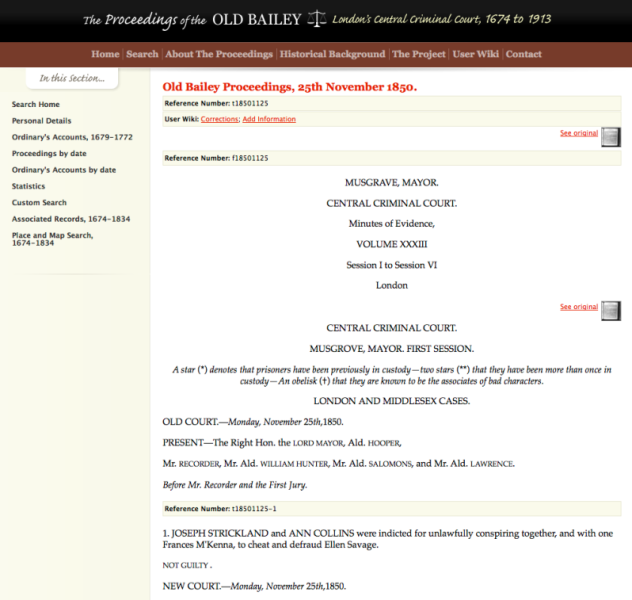
\includegraphics[keepaspectratio,width=\textwidth, height=.75\textheight]{images/oldbailey.png}
	\end{center}
	\end{figure}
	



\end{frame}
		

\begin{frame}
\frametitle{Perseus Digital Library}
\label{perseusdigitallibrary}

Virgil's {\itshape Aeneid}


\begin{figure}
	\label{aeneid}
	\begin{center}
	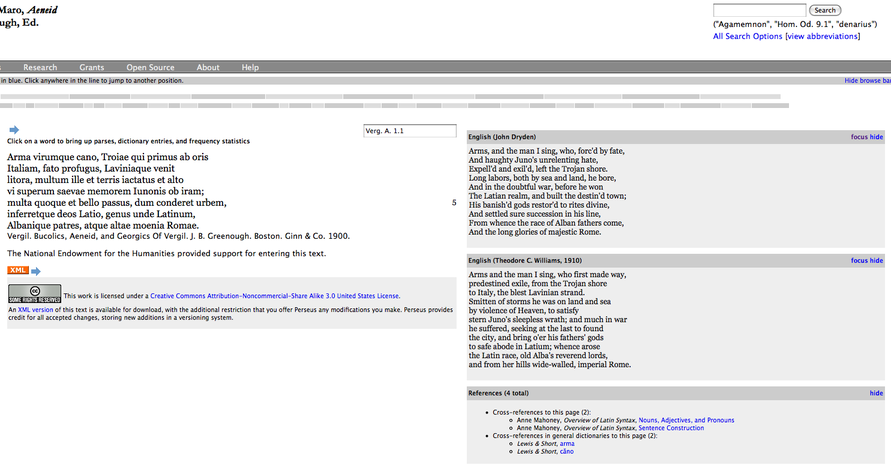
\includegraphics[keepaspectratio,width=\textwidth, height=.75\textheight]{images/aeneid60.png}
	\end{center}
	\end{figure}
	



\end{frame}
		

\begin{frame}
\frametitle{`Libraries': Literary and linguistic applications}
\label{libraries:literaryandlinguisticapplications}

Index Thomisticus (1946)


Perseus



\end{frame}
		

\begin{frame}
\frametitle{`Archives': Historical applications}
\label{archives:historicalapplications}

Digitisation


Data analysis


Collaboration



\end{frame}
		

\begin{frame}
\frametitle{Digitisation}
\label{digitisation}

Documents


Images


Linked/cross-referenced presentation of sources



\end{frame}
		

\begin{frame}
\frametitle{Tasmanian Police Gazette, 1861-1933}
\label{tasmanianpolicegazette1861-1933}

\begin{figure}
	\label{policegazette}
	\begin{center}
	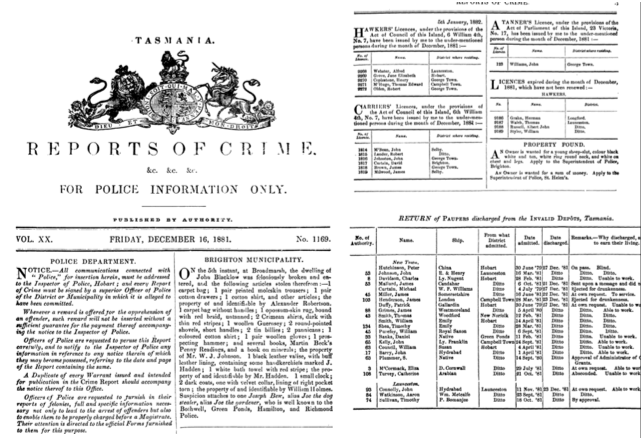
\includegraphics[keepaspectratio,width=\textwidth, height=.75\textheight]{images/police.png}
	\end{center}
	\end{figure}
	



\end{frame}
		

\begin{frame}
\frametitle{Surgeon's journals}
\label{surgeonsjournals}

\begin{figure}
	\label{marquisofhastingsjournal}
	\begin{center}
	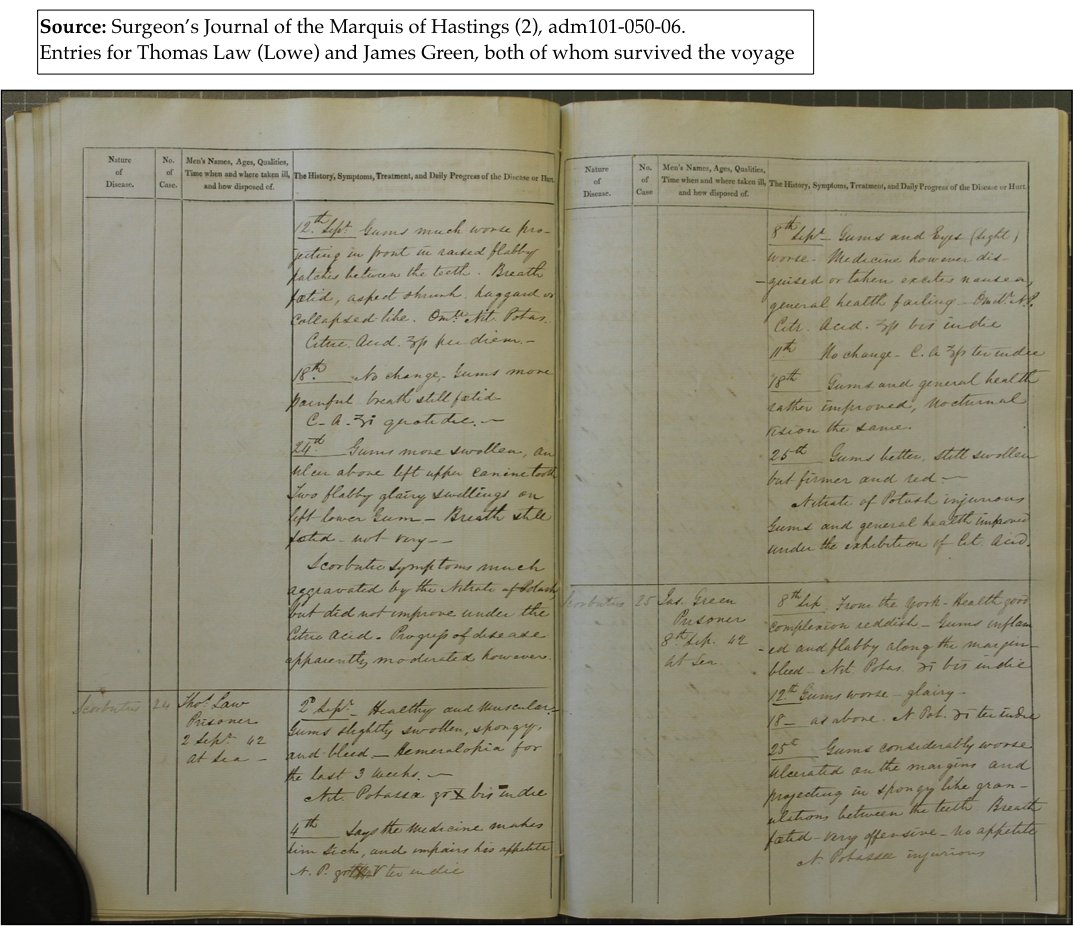
\includegraphics[keepaspectratio,width=\textwidth, height=.75\textheight]{images/journal.png}
	\end{center}
	\end{figure}
	



\end{frame}
		

\begin{frame}
\frametitle{Conduct registers}
\label{conductregisters}

\begin{figure}
	\label{marquisofhastingsconductrecord}
	\begin{center}
	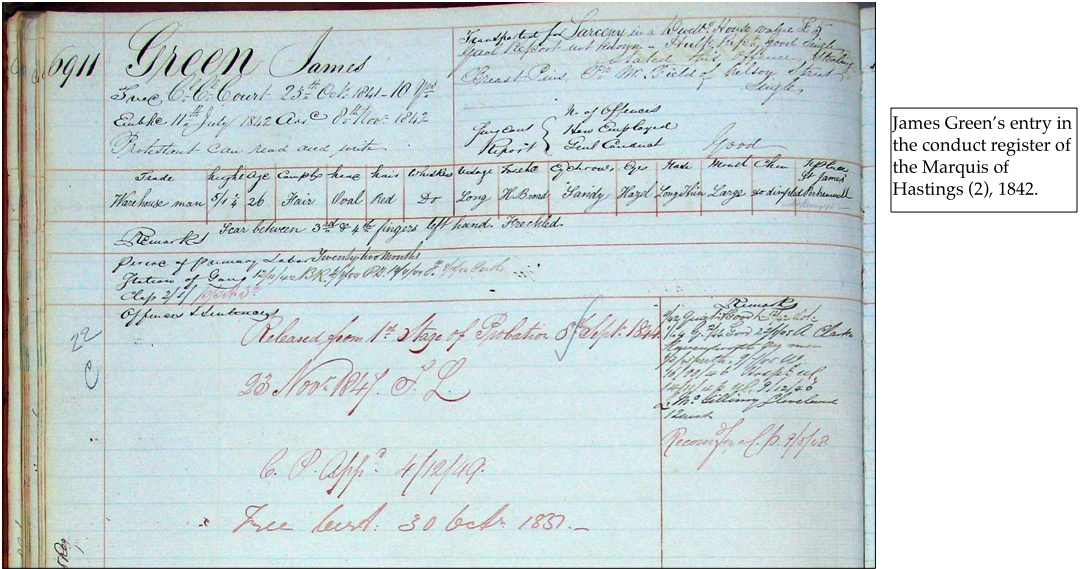
\includegraphics[keepaspectratio,width=\textwidth, height=.75\textheight]{images/conduct.png}
	\end{center}
	\end{figure}
	



\end{frame}
		

\begin{frame}
\frametitle{Data analysis}
\label{dataanalysis}

\begin{figure}
	\label{deathrates}
	\begin{center}
	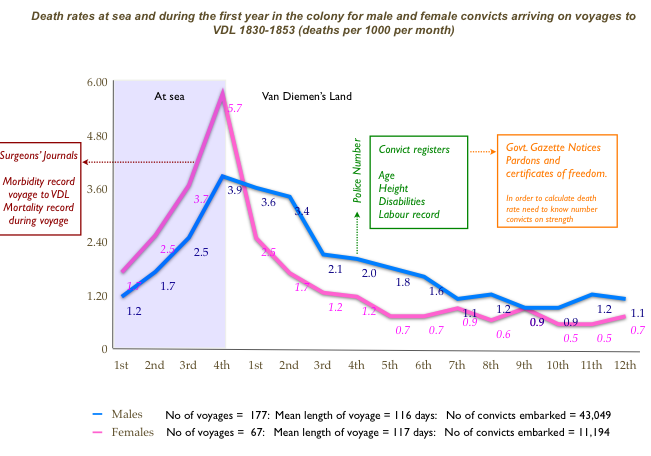
\includegraphics[keepaspectratio,width=\textwidth, height=.75\textheight]{images/deathrates.png}
	\end{center}
	\end{figure}
	



\end{frame}
		

\begin{frame}
\frametitle{GIS}
\label{gis}

\begin{figure}
	\label{mappingouranzacs}
	\begin{center}
	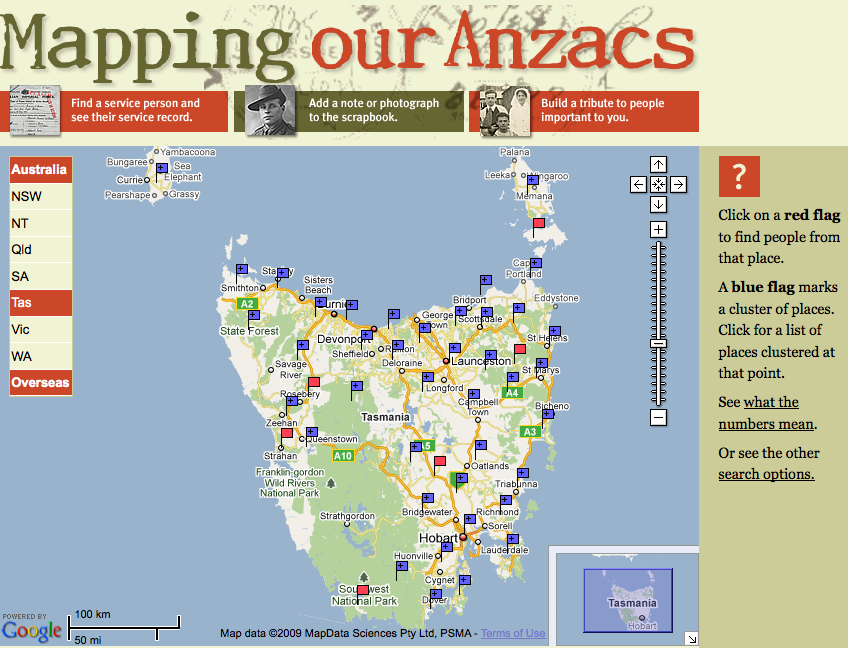
\includegraphics[keepaspectratio,width=\textwidth, height=.75\textheight]{images/mapping.png}
	\end{center}
	\end{figure}
	



\end{frame}
		

\begin{frame}
\frametitle{Collaboration}
\label{collaboration}

\begin{figure}
	\label{hobarttowngazette}
	\begin{center}
	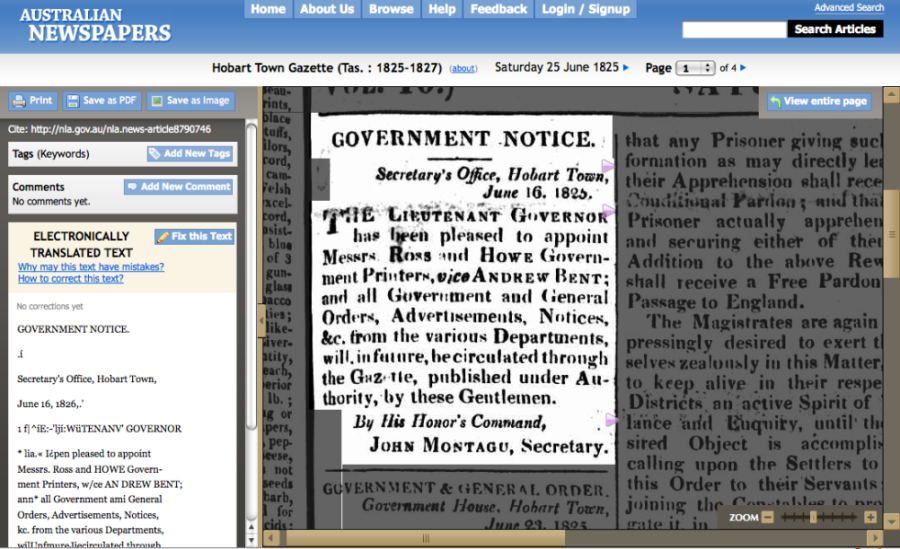
\includegraphics[keepaspectratio,width=\textwidth, height=.75\textheight]{images/htg.png}
	\end{center}
	\end{figure}
	



\end{frame}
		

\section{Why FOSS?}
\label{whyfoss}

\begin{frame}
\frametitle{Why FOSS?}
\label{whyfoss}

Use of resources


Community of developers


Using and adapting tools


Access


Values



\end{frame}
		

\begin{frame}
\frametitle{Use of resources}
\label{useofresources}

Expenses:


\begin{itemize}


\item Processing power

\item Storage

\item Bandwidth
\end{itemize}


\end{frame}
		

\begin{frame}
\frametitle{Community of developers}
\label{communityofdevelopers}

Mutual support


Don't reinvent the wheel


Using and adapting tools



\end{frame}
		

\begin{frame}
\frametitle{Access}
\label{access}

Make archival sources and research results accessible to general public


Sharing data with other researchers



\end{frame}
		

\begin{frame}
\frametitle{Values}
\label{values}

Public interest


Free access, free expression


Dialogue


Public participation



\end{frame}
		

\section{Challenges}
\label{challenges}

\begin{frame}
\frametitle{The Two Cultures}
\label{thetwocultures}

{\itshape The Two Cultures and the Scientific Revolution}


CP Snow, Rede Lecture, 1959


Literature/humanities vs science/tech



\end{frame}
		

\begin{frame}
\frametitle{Many cultures?}
\label{manycultures}

Translating between academics, IT professionals, diverse public audience


Different priorities, research questions



\end{frame}
		

\begin{frame}
\frametitle{Geeks and non-geeks}
\label{geeksandnon-geeks}

Non-geeks may not understand the values behind FOSS


Technology as magic



\end{frame}
		

\begin{frame}
\frametitle{Where do developers belong?}
\label{wheredodevelopersbelong}

Identity crisis


`Digital humanities professional'?


Background -- IT or academic?


Autonomy


Career progression


Where do humanities computing projects belong?



\end{frame}
		

\section{Data migration}
\label{datamigration}

\begin{frame}
\frametitle{From paper to digital}
\label{frompapertodigital}

\begin{figure}
	\label{marquisofhastingsconductrecord}
	\begin{center}
	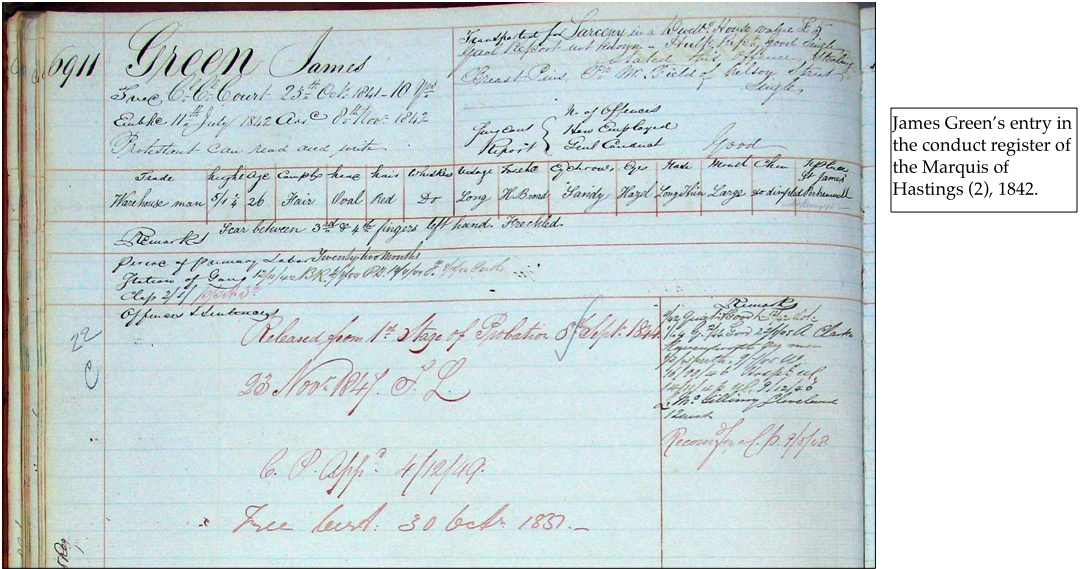
\includegraphics[keepaspectratio,width=\textwidth, height=.75\textheight]{images/conduct.png}
	\end{center}
	\end{figure}
	



\end{frame}
		

\begin{frame}
\frametitle{Screenshot: Index record}
\label{screenshot:indexrecord}

TODO



\end{frame}
		

\begin{frame}
\frametitle{Why Drupal?}
\label{whydrupal}

Modular


Define our own content types and views


Define user roles


Workflow



\end{frame}
		

\begin{frame}
\frametitle{Index data}
\label{indexdata}

Access --$>$ Excel --$>$ CSV


--$>$ Drupal?


Database on the web



\end{frame}
		

\begin{frame}
\frametitle{Content Construction Kit}
\label{contentconstructionkit}

TODO URL


Define your own data structures in Drupal


TODO screenshot



\end{frame}
		

\begin{frame}
\frametitle{Rules}
\label{rules}

\url{http://drupal.org/project/rules}


More powerful than core Trigger and Action modules


Generate a title for each node


\texttt{\{index number\} | \{convict name\} (\{ship name\})}



\end{frame}
		

\begin{frame}
\frametitle{Views}
\label{views}

TODO URL


Define your own views of content



\end{frame}
		

\begin{frame}
\frametitle{Table Wizard}
\label{tablewizard}

\url{http://drupal.org/project/tw}


Expose a MySQL table or CSV file to Views



\end{frame}
		

\begin{frame}
\frametitle{Table analysis}
\label{tableanalysis}

TODO local copy of Skitch screenshot


http://img.skitch.com/20100217-q5fi5t93y2nnr6p6jr3ks4isae.jpg



\end{frame}
		

\begin{frame}
\frametitle{Migrate}
\label{migrate}

\url{http://drupal.org/project/migrate}


Map structure of external table to a Drupal data structure


Migrate Extras \url{http://drupal.org/project/migrate\_extras} to migrate to CCK fields



\end{frame}
		

\begin{frame}
\frametitle{Content set}
\label{contentset}

TODO local copy of Skitch screenshot


http://img.skitch.com/20100217-mr3kkyq8gqmg4wumnqw844a387.jpg



\end{frame}
		

\begin{frame}
\frametitle{Migrate dashboard}
\label{migratedashboard}

TODO local copy of Skitch screenshot


http://img.skitch.com/20100217-t937n4rq5tqx1iqqxhdqne5gn.jpg



\end{frame}
		

\begin{frame}
\frametitle{Drush}
\label{drush}

Web-based dashboard good for testing on small samples


Drush: the Drupal Shell \url{http://drupal.org/project/drush}


(out of memory issues)


Run \texttt{drush migrate-import \{content set\}} from cron


Approx. one week to migrate \ensuremath{\sim} 80,000 records



\end{frame}
		

\section{Where to from here?}
\label{wheretofromhere}

\begin{frame}
\frametitle{Next stage of project}
\label{nextstageofproject}

(manually) linking official index with public submissions


\begin{itemize}


\item later life stories

\item WWI links
\end{itemize}


\end{frame}
		

\begin{frame}
\frametitle{Links}
\label{links}

The Valley of the Shadow \url{http://valley.lib.virginia.edu/}


Old Bailey Online \url{http://www.oldbaileyonline.org/}


Perseus Digital Library \url{http://www.perseus.tufts.edu/}


Index Thomisticus \url{http://www.corpusthomisticum.org/it/}



\end{frame}
		

\begin{frame}
\frametitle{Links}
\label{links}

Founders and Survivors \url{http://www.foundersandsurvivors.org/}


Mapping Our Anzacs \url{http://mappingouranzacs.naa.gov.au/}


Australian Newspapers (National Library) \url{http://newspapers.nla.gov.au/}


Essays in Humanities Computing \url{http://www.digitalhumanities.org/Essays/}



\end{frame}
		

\begin{frame}
\frametitle{Questions/advice?}
\label{questionsadvice}

\url{http://www.foundersandsurvivors.org/}


\url{http://www.slideshare.net/claudinec}



\end{frame}
		


%		\begin{frame}[allowframebreaks]
%\frametitle{Bibliography}

%	Bibliography
%\bibliographystyle{\mybibliostyle}
%\bibliocommand
%\end{frame}

\end{document}
